\documentclass{beamer}
\usetheme{Madrid}
\usecolortheme{seahorse}
\setbeamertemplate{navigation symbols}{}
\setbeamertemplate{footline}[frame number]
\usepackage{tikz}
\usetikzlibrary{shapes,arrows,positioning}
\usepackage{amsmath}
\usepackage{multirow}
\usepackage{graphicx}

\title{Smart Scheduling of Electric Vehicle Charging: Balancing Cost and User Satisfaction}
\author{Ankit Kumar Singh \\ 2021IMT-012 \\ Supervisor: Dr. Avadh Kishor}
\institute{ABV–IIITM Gwalior}
\date{\today}

\begin{document}

% Title
\begin{frame}
  \titlepage
\end{frame}

% Outline
\begin{frame}{Outline}
  \begin{enumerate}
    \item Introduction
    \item Background and Motivation
    \item Literature Review
    \item Research Gaps
    \item Model Architecture
    \item Methodology
    \begin{itemize}
        \item Priority Scheduling (Stage-I)
        \item Optimization (Stage-II)
    \end{itemize}
    \item Results and Analysis
    \item References
  \end{enumerate}
\end{frame}

% ============================================================
% Introduction (1 page / 2 frames)
% ============================================================
\section{Introduction}
\begin{frame}{Introduction}
  \begin{itemize}
    \item Rapid adoption of electric vehicles (EVs) is transforming transport and energy sectors globally.
    \item Global EV sales have shown exponential growth, with projections indicating approximately \textbf{200 million EVs} on roads by 2030 (IEA, 2023).
    \item Uncoordinated EV charging can lead to:
    \begin{itemize}
        \item Grid load congestion and voltage instability.
        \item Increased electricity costs for consumers.
        \item Accelerated battery degradation from aggressive charging cycles.
    \end{itemize}
    \item Smart charging and Vehicle-to-Grid (\textbf{V2G}) technologies offer grid support and cost saving opportunities.
    \item \textbf{Challenge}: Develop a multi-objective optimization framework that \textit{jointly} minimizes charging cost, battery degradation, and grid load variance while maximizing user satisfaction --- under limited charger availability and stochastic EV arrivals.
  \end{itemize}
\end{frame}

\begin{frame}{Problem Statement}
  \begin{block}{Core Problem}
  Given $N$ EVs competing for $M$ charging points ($N \gg M$) over a 12-hour horizon discretized into $T = 48$ time slots, determine:
  \begin{enumerate}
      \item \textbf{Which} EVs to admit (Stage-I: Priority Scheduling)
      \item \textbf{How much} power to assign (Stage-II: GA Optimization)
  \end{enumerate}
  such that total cost, degradation, and grid variance are minimized while user satisfaction is maximized.
  \end{block}
  \vspace{0.3cm}
  \textbf{Key Constraints}:
  \begin{itemize}
      \item Bidirectional charging: $P_{dis,min} \leq p_{i,t} \leq P_{ch,max}$
      \item SoC bounds: $0 \leq SoC_i(t) \leq 1$
      \item Grid capacity limit: $\sum_i p_{i,t} \leq P_{max}$
      \item Charger occupancy: At most $M$ EVs actively charging per slot
  \end{itemize}
\end{frame}

% ============================================================
% Background & Motivation
% ============================================================
\section{Background and Motivation}
\begin{frame}{Background}
  \begin{itemize}
    \item Global EV charging infrastructure expansion enables large-scale adoption.
    \item EVs act as energy consumers and grid-supporting storage units.
    \item Scheduling must address cost, user satisfaction, battery health, and grid constraints.
    \item Environmental impact: reduces emissions, supports cleaner grids.
  \end{itemize}
\end{frame}
\begin{frame}{Motivation}
  \begin{itemize}
    \item Reduce operational costs using bidirectional charging (V2G \& G2V).
    \item Extend battery lifespan by minimizing unnecessary cycling and degradation.
    \item Enhance user satisfaction by meeting charging preferences.
    \item Support grid stability and feasibility in real-world scenarios.
  \end{itemize}
\end{frame}

% ============================================================
% Literature Review
% ============================================================
\section{Literature Review}
\begin{frame}{Literature Review: Methods}
  \begin{itemize}
    \item \textbf{Linear programming (LP)}: Effective for EV charging with linear objectives/constraints (e.g., TOU pricing).
    \item \textbf{Dynamic programming (DP)}: Optimal for sequential decision-making but suffers from curse of dimensionality.
    \item \textbf{Mixed Integer Linear Programming (MILP)}: Handles continuous/discrete variables; computationally intensive for large fleets.
    \item \textbf{Metaheuristic algorithms}: GA, PSO, GSA are promising for non-convex optimization.
  \end{itemize}
\end{frame}

\begin{frame}{Literature Review: Key Factors}
  \begin{itemize}
    \item \textbf{Cost}: TOU pricing enables up to 75\% cost reduction by shifting load (Off-peak charging).
    \item \textbf{Battery Health}: Degradation depends on Temperature, SoC, C-rate; optimized strategies extend life by ~25\%.
    \item \textbf{User Satisfaction}: Modeled via utility functions (SoC at departure, deadline compliance).
    \item \textbf{Fairness}: Resource allocation fairness measured by Coefficient of Variation (CV).
  \end{itemize}
\end{frame}

\begin{frame}{Literature Review Summary}
  \footnotesize
  \begin{tabular}{|p{2.5cm}|p{2.5cm}|p{2.5cm}|p{2.5cm}|}
    \hline
    \textbf{Author (Year)} & \textbf{Method} & \textbf{Pros} & \textbf{Gaps} \\
    \hline
    Bhaskar et al. (2024) & V2G/G2V Scheduling & Balances Cost/Aging & Scalability issues \\
    \hline
    Tan et al. (2023) & Multi-Agent + GA & Autonomous & Complexity \\
    \hline
    Pan et al. (2024) & Hybrid IGSAPSO & Efficient Balancing & Data intensive \\
    \hline
    Fernandes (2017) & On-Off Scheduling & Fast & No user comfort \\
    \hline
    Wu et al. (2022) & Online Greedy & Fast & Peak issues \\
    \hline
  \end{tabular}
\end{frame}

% ============================================================
% Research Gaps (2 pages / 2 frames)
% ============================================================
\section{Research Gaps}
\begin{frame}{Research Gaps: Methodology Limitations}
  \begin{itemize}
    \item \textbf{Oversimplified Trade-offs}: Most studies optimize a single objective (cost or grid stability) or decouple cost minimization from user satisfaction, ignoring the inherent multi-objective nature of the problem.
    \item \textbf{Stochasticity Ignored}: Many formulations assume deterministic EV arrival/departure patterns, ignoring real-world randomness in arrival times, initial SoC, and time-of-use price fluctuations.
    \item \textbf{Scalability}: Exact optimization methods (LP, MILP, DP) struggle with large EV fleets ($N > 100$) due to exponential computational complexity.
    \item \textbf{Fixed Charger Assignment}: Most frameworks do not address dynamic charger reassignment --- once an EV is plugged in, it occupies the charger until departure regardless of whether its target SoC has been met.
  \end{itemize}
\end{frame}

\begin{frame}{Research Gaps: System-Level Limitations}
  \begin{itemize}
    \item \textbf{Holistic Framework Missing}: No existing work \textit{jointly} models all four objectives --- Cost, User Satisfaction, Battery Degradation, and Grid Load Variance --- within a single optimization framework.
    \item \textbf{Battery Degradation Modeling}: Many studies use simplistic degradation models that ignore the energy throughput based aging mechanism ($c_{deg} \cdot |p_{i,t}| \cdot \Delta\delta$).
    \item \textbf{Limited Charger Scenarios}: Most studies assume unlimited or abundant chargers ($M \geq N$), which is unrealistic in workplace or urban parking scenarios where $N \gg M$.
    \item \textbf{No Priority-Based Admission}: Existing methods lack a systematic priority scoring mechanism to decide \textit{which} EVs should be admitted when chargers are scarce --- they either use FCFS or random admission.
  \end{itemize}
  \vspace{0.3cm}
  \begin{block}{Our Contribution}
  A Two-Stage framework integrating \textbf{Priority Scheduling} (Stage-I) with \textbf{GA-based Power Optimization} (Stage-II) addressing all identified gaps.
  \end{block}
\end{frame}

% ============================================================
% Model Architecture
% ============================================================
\section{Model Architecture}
\begin{frame}{System Model Architecture}
  \centering
  \resizebox{0.9\textwidth}{!}{
  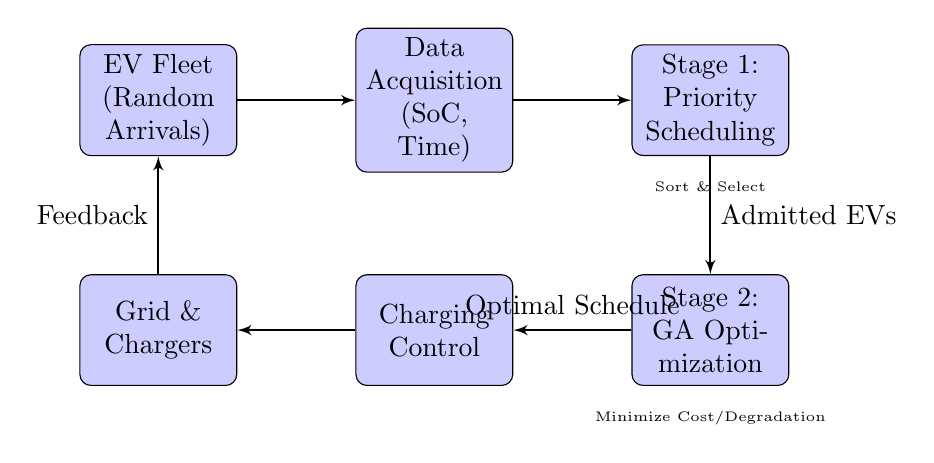
\begin{tikzpicture}[node distance=2cm, auto,
    block/.style={rectangle, draw, fill=blue!20, text width=5em, text centered, rounded corners, minimum height=4em},
    line/.style={draw, -latex', thick},
    cloud/.style={draw, ellipse, fill=red!20, node distance=3cm, minimum height=2em}]
    
    % Nodes
    \node [block] (evs) {EV Fleet (Random Arrivals)};
    \node [block, right=1.5cm of evs] (data) {Data Acquisition (SoC, Time)};
    \node [block, right=1.5cm of data] (stage1) {Stage 1: Priority Scheduling};
    \node [block, below=1.5cm of stage1] (stage2) {Stage 2: GA Optimization};
    \node [block, left=1.5cm of stage2] (control) {Charging Control};
    \node [block, left=1.5cm of control] (grid) {Grid \& Chargers};

    % Edges
    \path [line] (evs) -- (data);
    \path [line] (data) -- (stage1);
    \path [line] (stage1) -- node[midway, right] {Admitted EVs} (stage2);
    \path [line] (stage2) -- node[midway, above] {Optimal Schedule} (control);
    \path [line] (control) -- (grid);
    \path [line] (grid) -- node[midway, left] {Feedback} (evs);
    
    % Annotations
    \node [below=0.2cm of stage1, font=\tiny] {Sort \& Select};
    \node [below=0.2cm of stage2, font=\tiny] {Minimize Cost/Degradation};
  \end{tikzpicture}
  }
  \caption{Two-Stage Smart Scheduling Framework}
\end{frame}

% ============================================================
% Methodology
% ============================================================
\section{Methodology}
\begin{frame}{Methodology Overview}
  We propose a \textbf{Two-Stage Hierarchical Approach}:
  \vspace{0.5cm}
  \begin{itemize}
      \item \textbf{Stage I: Priority-Based Scheduling}
      \begin{itemize}
          \item Handles resource constraints (Limited Chargers vs. Many EVs).
          \item Assigns priority based on Urgency, Degradation, Grid Stress, and Price.
      \end{itemize}
      \item \textbf{Stage II: Genetic Algorithm (GA) Optimization}
      \begin{itemize}
          \item Optimizes charging power profiles for admitted EVs.
          \item Multi-objective: Cost, Battery Health, Grid Variance, Satisfaction.
      \end{itemize}
  \end{itemize}
\end{frame}

\subsection{Stage I: Priority Scheduling}
\begin{frame}{Stage I: Priority Factors}
  We calculate four normalized factors for each waiting EV $i$ to determine its charging priority. The factors are evaluated in the following order of influence:

  \begin{enumerate}
      \item \textbf{Price Factor ($P_i$)}: Incentivizes charging during low-price periods.
      $$ P_i = \frac{\pi_{buy}(t) - \pi_{min}}{\pi_{max} - \pi_{min}} $$
      \item \textbf{Degradation Cost Factor ($D_i$)}: Penalizes battery aging costs.
      $$ D_i = \frac{(C_{deg} \cdot \Delta E_i) - D_{min}}{D_{max} - D_{min}} $$
      \item \textbf{Grid Stress Factor ($G_i$)}: Penalizes charging when grid load is high.
      $$ G_i = \max\left(0, \frac{\sum P_{req} - P_{avg}}{P_{max} - P_{avg}}\right) $$
      \item \textbf{User Satisfaction / Urgency ($\phi_i$)}: Ensures deadline compliance.
      $$ \phi_i = \min\left(1, \frac{P_{req,i}}{P_{ref}}\right), \quad \text{where } P_{req,i} = \frac{SoC_{max} - SoC_{curr}}{T_{remain}} \cdot E_{cap} $$
  \end{enumerate}
\end{frame}

\begin{frame}{Stage I: Priority Score \& Admission}
  The final \textbf{Priority Score ($\lambda_i$)} is calculated by aggregating these factors. A higher $\lambda_i$ implies higher priority for charger allocation.
  
  \begin{block}{Priority Function}
  $$ \lambda_i = w_s \cdot \phi_i - w_p \cdot P_i - w_d \cdot D_i - w_g \cdot G_i $$
  \end{block}

  \textbf{Interpretation}:
  \begin{itemize}
      \item \textbf{Positive Term ($w_s \phi_i$)}: Increases priority for urgent EVs.
      \item \textbf{Negative Terms}: Reduce priority if Price ($P_i$), Degradation ($D_i$), or Grid Stress ($G_i$) are high.
  \end{itemize}

  \textbf{Selection}: Sort EVs by $\lambda_i$ descending; the top $M$ EVs are admitted.
\end{frame}

\subsection{Stage II: Optimization}
\begin{frame}{Stage II: GA Optimization Objective}
  We minimize a multi-objective cost function $J$ for the admitted EVs:
  
  $$ \min J = w_1 F_1 + w_2 F_2 + w_3 F_3 - w_4 F_4 + \Omega_{penalty} $$
  
  \begin{itemize}
      \item $F_1$: \textbf{Operational Cost} (Time-of-Use Energy Cost).
      $$ F_1 = \sum_{t} \sum_{i} \left( \pi_{buy}(t) P_{ch}(i,t) + \pi_{rev}(t) P_{dis}(i,t) \right) \Delta t $$
      \item $F_2$: \textbf{Battery Degradation Cost}.
      $$ F_2 = \sum_{t} \sum_{i} c_{deg} |P(i,t)| \Delta t $$
  \end{itemize}
\end{frame}

\begin{frame}{Stage II: Optimization Objectives (Cont.)}
  \begin{itemize}
      \item $F_3$: \textbf{Grid Load Variance} (Peak Shaving).
      $$ F_3 = \sum_{t} \left( L(t) - L_{avg} \right)^2, \quad L(t) = \sum_i P(i,t) $$
      \item $F_4$: \textbf{User Satisfaction} (Maximize SoC).
      $$ F_4 = \sum_{i} S_i, \quad S_i = \max\left(0, 1 - \phi_i \frac{SoC_{max} - SoC_{final,i}}{SoC_{max} - SoC_{init}}\right) $$
      \item $\Omega_{penalty}$: Penalties for constraints violation (Power limits, Grid Capacity $P_{max}$, SoC limits).
  \end{itemize}
\end{frame}

\begin{frame}{Stage II: Evolutionary Process}
  \textbf{Genetic Algorithm (GA) Configuration}:
  \begin{itemize}
      \item \textbf{Encoding}: Real-valued vector representing Power $P(i,t)$ for all admitted EVs and Time Slots.
      \item \textbf{Crossover}: Simulated Binary Crossover (SBX).
      \item \textbf{Mutation}: Polynomial Mutation to introduce small variations.
      \item \textbf{Selection}: Tournament Selection.
      \item \textbf{Repair Mechanism}: Heuristic repair to ensure $P_{min} \le P(i,t) \le P_{max}$ and stay within SoC bounds.
  \end{itemize}
\end{frame}

% ============================================================
% Results and Analysis (3 pages / 5 frames)
% ============================================================
\section{Results and Analysis}

\begin{frame}{Experimental Setup}
  \begin{itemize}
      \item \textbf{Scenario}: Workplace parking lot with $M = 10$ bidirectional chargers, 12-hour horizon (8 AM--8 PM), $T = 48$ slots of 15 min each.
      \item \textbf{Fleet sizes tested}: $N \in \{50, 100, 150, 200, 250, 300\}$ EVs.
      \item \textbf{Baselines}: First-Come-First-Serve (FCFS) and Shortest-Job-First (SJF).
      \item \textbf{GA parameters}: Population $= 120$, Generations $= 300$, $p_c = 0.9$, $p_m = 0.3$, $\eta_c = \eta_m = 20$, Tournament size $= 3$.
      \item \textbf{Objective weights}: $w_1 = w_2 = w_3 = w_4 = 0.25$.
  \end{itemize}
  \vspace{0.3cm}
  \textbf{Sensitivity experiments} conducted on:
  \begin{enumerate}
      \item Charger Power Mix (Slow / Medium / Fast)
      \item Fleet Composition (Compact vs. SUV ratio)
      \item Initial SoC Distribution (Low / Moderate / High)
  \end{enumerate}
\end{frame}

\begin{frame}{Performance Comparison: Cost \& Degradation}
  \begin{table}[]
  \centering
  \footnotesize
  \begin{tabular}{|c|c|c|c|c|c|c|}
  \hline
  \multirow{2}{*}{\textbf{N}} & \multicolumn{3}{c|}{\textbf{Avg. Cost (\$/EV)}} & \multicolumn{3}{c|}{\textbf{Avg. Degradation (\$/EV)}} \\
  \cline{2-7}
   & \textbf{FCFS} & \textbf{SJF} & \textbf{Proposed} & \textbf{FCFS} & \textbf{SJF} & \textbf{Proposed} \\
  \hline
  50  & 1.88 & $-$0.26 & \textbf{0.95} & 0.184 & 0.061 & \textbf{0.098} \\
  \hline
  100 & 3.76 & 0.50  & \textbf{0.86} & 0.416 & 0.089 & \textbf{0.099} \\
  \hline
  150 & 4.35 & $-$0.46 & \textbf{0.75} & 0.427 & 0.125 & \textbf{0.087} \\
  \hline
  200 & 4.07 & $-$0.22 & \textbf{0.55} & 0.399 & 0.064 & \textbf{0.049} \\
  \hline
  250 & 3.99 & $-$0.20 & \textbf{0.44} & 0.360 & 0.115 & \textbf{0.049} \\
  \hline
  300 & 4.18 & $-$0.97 & \textbf{0.33} & 0.342 & 0.152 & \textbf{0.037} \\
  \hline
  \end{tabular}
  \caption{Cost and Degradation across fleet sizes}
  \end{table}
  \textbf{Key findings}:
  \begin{itemize}
      \item Proposed method achieves \textbf{86--92\%} cost reduction vs. FCFS.
      \item Degradation reduced by \textbf{$\approx$87\%} by avoiding aggressive micro-cycles.
      \item Cost per EV \textit{decreases} with larger fleets --- economies of scale.
  \end{itemize}
\end{frame}

\begin{frame}{Performance Comparison: Grid \& Waiting Time}
  \begin{table}[]
  \centering
  \footnotesize
  \begin{tabular}{|c|c|c|c|c|c|c|}
  \hline
  \multirow{2}{*}{\textbf{N}} & \multicolumn{3}{c|}{\textbf{Grid Variance (kW$^2$)}} & \multicolumn{3}{c|}{\textbf{Avg. Waiting Time (slots)}} \\
  \cline{2-7}
   & \textbf{FCFS} & \textbf{SJF} & \textbf{Proposed} & \textbf{FCFS} & \textbf{SJF} & \textbf{Proposed} \\
  \hline
  50  & 20,754  & \textbf{5,617}  & 17,532  & \textbf{2.80} & 2.55  & 3.71  \\
  \hline
  100 & 55,368  & \textbf{2,460}  & 39,602  & 4.13 & \textbf{4.08} & 3.18  \\
  \hline
  150 & 77,339  & \textbf{4,737}  & 57,579  & 4.91 & 4.87 & \textbf{4.29}  \\
  \hline
  200 & 74,957  & \textbf{2,961}  & 50,354  & 5.03 & 4.97 & \textbf{4.53}  \\
  \hline
  250 & 58,402  & \textbf{3,640}  & 43,548  & 5.01 & 5.02 & \textbf{4.70}  \\
  \hline
  300 & 59,743  & \textbf{10,012} & 42,086  & 5.06 & 5.04 & \textbf{4.80}  \\
  \hline
  \end{tabular}
  \caption{Grid Load Variance and Waiting Time comparison}
  \end{table}
  \textbf{Key findings}:
  \begin{itemize}
      \item Grid variance reduced by \textbf{33--44\%} vs. FCFS --- smoother load profile.
      \item For $N \geq 150$, proposed method achieves \textbf{lowest waiting time} via efficient charger reallocation.
  \end{itemize}
\end{frame}

\begin{frame}{Combined Comparison \& Convergence}
  \begin{columns}[T]
    \begin{column}{0.48\textwidth}
      \centering
      
\includegraphics[width=\textwidth]{results_figures/comparison_combined.png}
      \\ \footnotesize All metrics across fleet sizes
    \end{column}
    \begin{column}{0.48\textwidth}
      \centering
      
\includegraphics[width=\textwidth]{results_figures/convergence_plot_ev_variations.png}
      \\ \footnotesize GA convergence ($N = 20$ to $100$)
    \end{column}
  \end{columns}
  \vspace{0.3cm}
  \begin{itemize}
      \item \footnotesize Proposed framework \textbf{consistently outperforms} FCFS across cost, degradation, and grid variance.
      \item \footnotesize GA converges reliably within $\sim$50--150 generations; early stopping ensures efficiency.
  \end{itemize}
\end{frame}

\begin{frame}{Sensitivity Analysis Summary}
  \footnotesize
  \begin{table}[]
  \centering
  \begin{tabular}{|l|c|c|c|}
  \hline
  \textbf{Experiment} & \textbf{FCFS Cost (\$)} & \textbf{Proposed Cost (\$)} & \textbf{Reduction} \\
  \hline
  \multicolumn{4}{|l|}{\textit{Charger Power Mix}} \\
  \hline
  Slow (3--5 kW)    & 4.27 & \textbf{1.37} & 68\% \\
  Medium (5--9 kW)   & 4.18 & \textbf{0.77} & 82\% \\
  Fast (9--15 kW)    & 4.66 & \textbf{0.50} & 89\% \\
  \hline
  \multicolumn{4}{|l|}{\textit{Fleet Composition}} \\
  \hline
  70\% Compact       & 4.52 & \textbf{0.94} & 79\% \\
  50\% Compact       & 5.02 & \textbf{$-$0.01} & $>$99\% \\
  30\% Compact       & 5.14 & \textbf{0.49} & 90\% \\
  \hline
  \multicolumn{4}{|l|}{\textit{Initial SoC Distribution}} \\
  \hline
  Low SoC            & 4.55 & \textbf{0.32} & 93\% \\
  Moderate SoC       & 4.76 & \textbf{0.85} & 82\% \\
  High SoC           & 4.17 & \textbf{0.29} & 93\% \\
  \hline
  \end{tabular}
  \caption{Sensitivity analysis: Cost reduction under varying conditions}
  \end{table}
  \normalsize
  \textbf{Conclusion}: The framework is \textbf{robust} across all sensitivity scenarios --- cost reduction ranges from \textbf{68\% to $>$99\%} vs. FCFS regardless of charger type, fleet mix, or initial SoC.
\end{frame}

% ============================================================
% References
% ============================================================
\section{References}
\begin{frame}{References}
  \footnotesize
  \begin{thebibliography}{99}
    \bibitem{bhaskar2024} Bhaskar, A., et al., ``Scheduling of Electric Vehicles Power in V2G and G2V Modes...'', IEEE Trans. Smart Grid, 2024.
    \bibitem{tan2023} Tan, M., et al., ``Multi-Agent System for Electric Vehicle Charging Scheduling...'', CSMS, 2023.
    \bibitem{pan2024} Pan, K., et al., ``Optimal Electric Vehicle Charge--Discharge Scheduling Using Hybrid IGSAPSO'', IJEPES 2024.
    \bibitem{fernandes2017} Fernandes, X., et al., ``On-Off Scheduling Schemes...'', 4OR-Q J Oper Res, 2017.
    \bibitem{wu2022} Wu, W., et al., ``Online EV Charge Scheduling'', IEEE T-ITS, 2022.
    \bibitem{nimalsiri2022} Nimalsiri, N., et al., ``Load Curve Shaping...'', IEEE T-ITS, 2022.
  \end{thebibliography}
\end{frame}

\begin{frame}[plain]
  \centering
  \vspace{2cm}
  {\Huge \textbf{Thank You}}
  
  \vspace{1cm}
  \large Questions?
\end{frame}

\end{document}
